\documentclass{article}
\usepackage{graphics} 
\usepackage{hyperref}

\author{Kevin Zollicoffer}
\title{Regression\\Lesson 1a}
\date{10/14/2013}

\usepackage{Sweave}
\begin{document}
\maketitle
%\tableofcontents
\Sconcordance{concordance:Assignment1A.tex:Assignment1A.Rnw:%
1 14 1 1 0 15 1}


\section*{Introduction}
Regression assignment 1a using R. 
\\
\\
The complete source for this assigment is available on Github:
\\
\\
\url{https://github.com/zollie/PASS-Regression-Assignment1a}

\section*{Problem 1.1}
\begin{Schunk}
\begin{Sinput}
>   nbas <- read.csv("~/R/PASS/Regression/Assignment1a/nbasalary.csv")
\end{Sinput}
\end{Schunk}

\subsection*{a}
\begin{Schunk}
\begin{Sinput}
> hist(nbas$Salary, freq=TRUE)
\end{Sinput}
\end{Schunk}
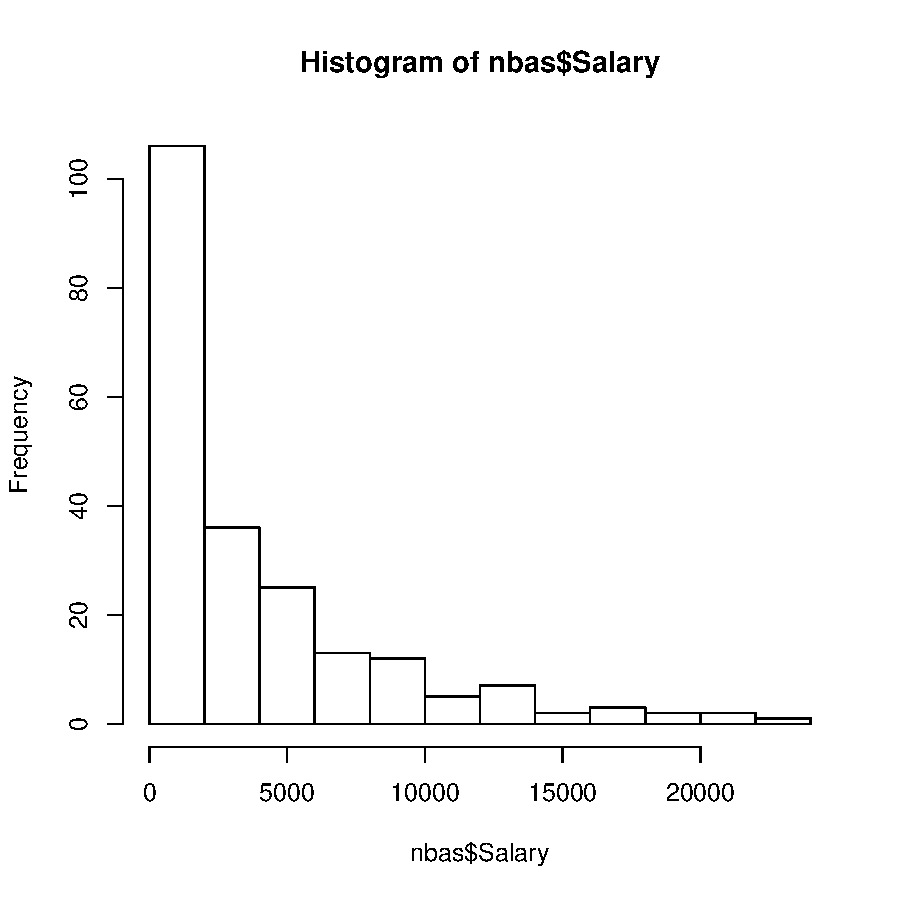
\includegraphics{Assignment1A-002}

\subsection*{b}
A bell curve like that of the standard normal distribution

\subsection*{c}
\begin{Schunk}
\begin{Sinput}
> qqnorm(nbas$Salary)
> qqline(nbas$Salary)
\end{Sinput}
\end{Schunk}
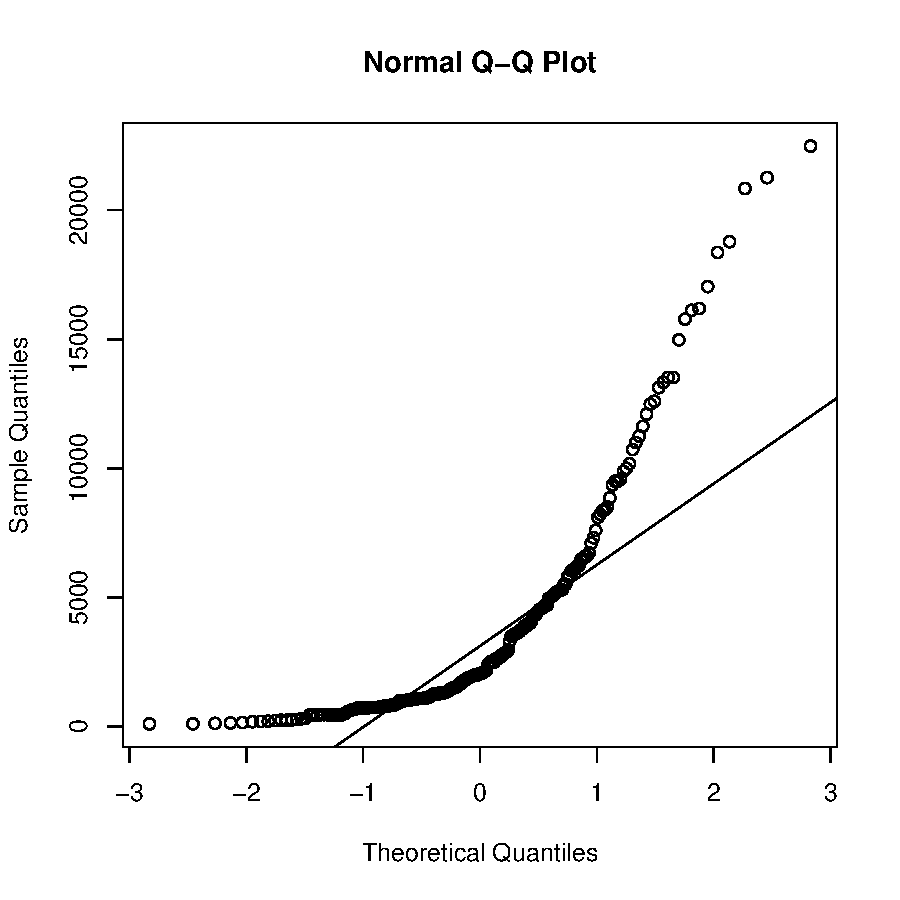
\includegraphics{Assignment1A-003}

\subsection*{d}
The QQ plot would be clustered around the reference line added by qqline()

\subsection*{e}
\begin{Schunk}
\begin{Sinput}
> Logsal <- log(nbas$Salary)
> hist(Logsal, freq=TRUE)
\end{Sinput}
\end{Schunk}
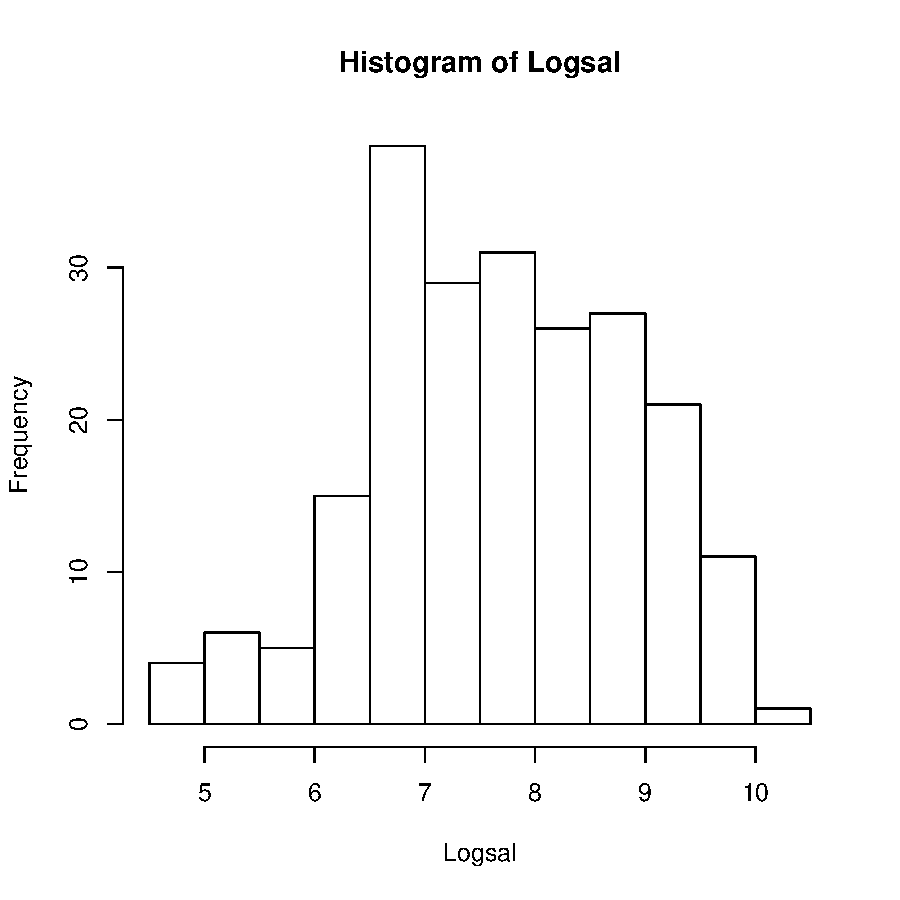
\includegraphics{Assignment1A-004}

\subsection*{f}
\begin{Schunk}
\begin{Sinput}
> qqnorm(Logsal)
> qqline(Logsal)
\end{Sinput}
\end{Schunk}
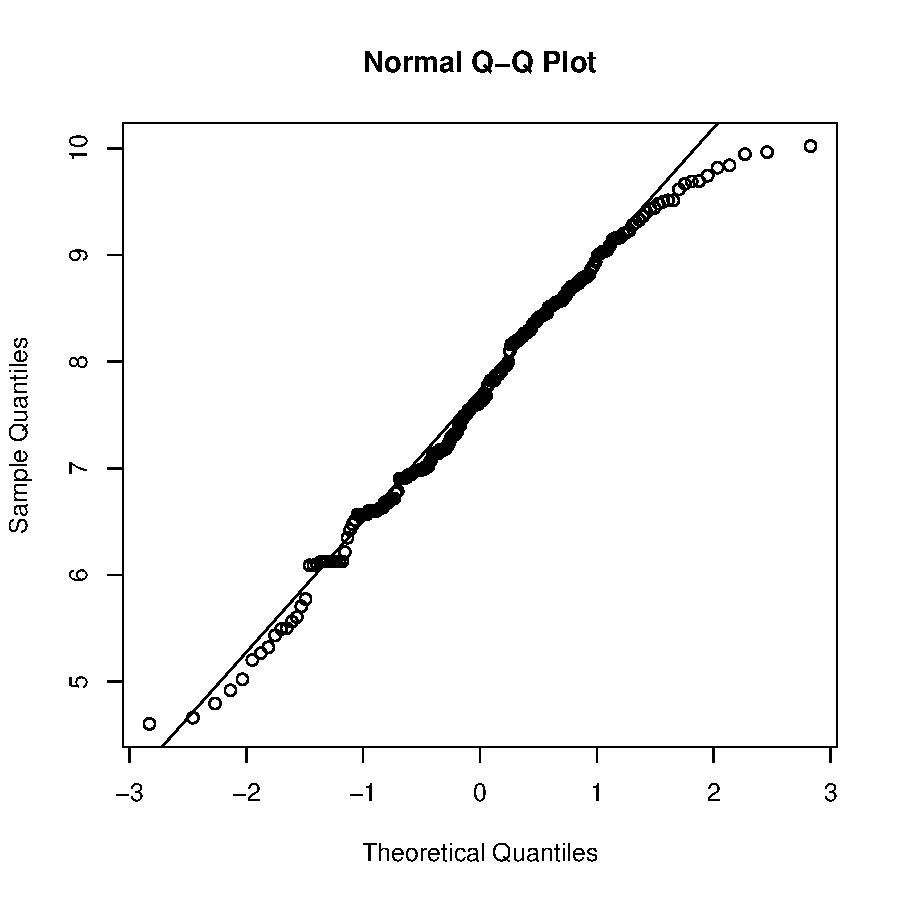
\includegraphics{Assignment1A-005}

\subsection*{g}
Logsal more closely follows a normal curve. The histogram of Logsal resembles the standard normal distribution more than the histogram of nbas\$Salaries. Likewise, the QQ-plot of Logsal clusters around the normal reference line to a greater degree than that of the qqplot of nbas\$Salaries. 

\section*{Problem 1.5}
\begin{Schunk}
\begin{Sinput}
>   c <- read.csv("~/R/PASS/Regression/Assignment1a/countries.csv")
\end{Sinput}
\end{Schunk}

\subsection*{a}
\begin{Schunk}
\begin{Sinput}
>   summary(c$Pop)
\end{Sinput}
\begin{Soutput}
   Min. 1st Qu.  Median    Mean 3rd Qu.    Max. 
  20.71   29.52   46.08  111.50   82.63 1341.00 
\end{Soutput}
\begin{Sinput}
>   mean(c$Pop)
\end{Sinput}
\begin{Soutput}
[1] 111.5442
\end{Soutput}
\begin{Sinput}
>   sd(c$Pop)
\end{Sinput}
\begin{Soutput}
[1] 237.241
\end{Soutput}
\end{Schunk}

\subsection*{b}
The world population among countries is highly variable about the mean as exhibited by a mean of 111.5 and a standard deviation of 237.2. That is c\$Pop is not normally distributed but highly skewed. Therefore the confidence intervals for the mean of c\$Pop would be relatively large and weakly informative. 

\subsection*{c}
\begin{Schunk}
\begin{Sinput}
> nrow(c)
\end{Sinput}
\begin{Soutput}
[1] 55
\end{Soutput}
\begin{Sinput}
> mean(c$Life)
\end{Sinput}
\begin{Soutput}
[1] 69.78702
\end{Soutput}
\begin{Sinput}
> sd(c$Life)
\end{Sinput}
\begin{Soutput}
[1] 9.250388
\end{Soutput}
\begin{Sinput}
> t.test(c$Life, conf.level=.95)
\end{Sinput}
\begin{Soutput}
	One Sample t-test

data:  c$Life
t = 55.9495, df = 54, p-value < 2.2e-16
alternative hypothesis: true mean is not equal to 0
95 percent confidence interval:
 67.28629 72.28775
sample estimates:
mean of x 
 69.78702 
\end{Soutput}
\end{Schunk}

\section*{Problem 1.7}
\subsection*{a}
\begin{Schunk}
\begin{Sinput}
> t.test(c$Life, mu=68, alternative="less")
\end{Sinput}
\begin{Soutput}
	One Sample t-test

data:  c$Life
t = 1.4327, df = 54, p-value = 0.9211
alternative hypothesis: true mean is less than 68
95 percent confidence interval:
     -Inf 71.87449
sample estimates:
mean of x 
 69.78702 
\end{Soutput}
\end{Schunk}
p-value > .05 therefore we do not reject the null hypothesis. The journalist may be correct in this scenario.

\subsection*{b}
The prediction intervals below are larger than the confidence intervals from problem 1.5c because when calculating a confidence interval the only error we have to worry about is the estimation error. However, when calculating a prediction interval we must account for the estimation error and random error. 

\subsubsection*{Manually}
\begin{Schunk}
\begin{Sinput}
> f <- function(d, conf) {
+   lwr <- mean(c$Life) - conf*sd(c$Life)*sqrt(1+1/length(c$Life))
+   upr <- mean(c$Life) + conf*sd(c$Life)*sqrt(1+1/length(c$Life))
+   c(lwr,upr)
+ }
> f(c$Life, 2.005)
\end{Sinput}
\begin{Soutput}
[1] 51.07214 88.50190
\end{Soutput}
\end{Schunk}

\subsubsection*{Regression Trick}
\begin{Schunk}
\begin{Sinput}
> ones <- rep(1, 55)
> model <- lm(c$Life ~ ones)
> predict(model, interval="prediction")
\end{Sinput}
\begin{Soutput}
        fit      lwr      upr
1  69.78702 51.07327 88.50077
2  69.78702 51.07327 88.50077
3  69.78702 51.07327 88.50077
4  69.78702 51.07327 88.50077
5  69.78702 51.07327 88.50077
6  69.78702 51.07327 88.50077
7  69.78702 51.07327 88.50077
8  69.78702 51.07327 88.50077
9  69.78702 51.07327 88.50077
10 69.78702 51.07327 88.50077
11 69.78702 51.07327 88.50077
12 69.78702 51.07327 88.50077
13 69.78702 51.07327 88.50077
14 69.78702 51.07327 88.50077
15 69.78702 51.07327 88.50077
16 69.78702 51.07327 88.50077
17 69.78702 51.07327 88.50077
18 69.78702 51.07327 88.50077
19 69.78702 51.07327 88.50077
20 69.78702 51.07327 88.50077
21 69.78702 51.07327 88.50077
22 69.78702 51.07327 88.50077
23 69.78702 51.07327 88.50077
24 69.78702 51.07327 88.50077
25 69.78702 51.07327 88.50077
26 69.78702 51.07327 88.50077
27 69.78702 51.07327 88.50077
28 69.78702 51.07327 88.50077
29 69.78702 51.07327 88.50077
30 69.78702 51.07327 88.50077
31 69.78702 51.07327 88.50077
32 69.78702 51.07327 88.50077
33 69.78702 51.07327 88.50077
34 69.78702 51.07327 88.50077
35 69.78702 51.07327 88.50077
36 69.78702 51.07327 88.50077
37 69.78702 51.07327 88.50077
38 69.78702 51.07327 88.50077
39 69.78702 51.07327 88.50077
40 69.78702 51.07327 88.50077
41 69.78702 51.07327 88.50077
42 69.78702 51.07327 88.50077
43 69.78702 51.07327 88.50077
44 69.78702 51.07327 88.50077
45 69.78702 51.07327 88.50077
46 69.78702 51.07327 88.50077
47 69.78702 51.07327 88.50077
48 69.78702 51.07327 88.50077
49 69.78702 51.07327 88.50077
50 69.78702 51.07327 88.50077
51 69.78702 51.07327 88.50077
52 69.78702 51.07327 88.50077
53 69.78702 51.07327 88.50077
54 69.78702 51.07327 88.50077
55 69.78702 51.07327 88.50077
\end{Soutput}
\end{Schunk}

\end{document}
